\documentclass[11pt,a4paper]{article}

\usepackage[utf8]{inputenc}
\usepackage[T1]{fontenc}
\usepackage{lmodern}
\usepackage{microtype}
\emergencystretch=3em
\usepackage[margin=2.6cm]{geometry}
\usepackage{amsmath,amssymb,amsthm,mathtools}
\usepackage{booktabs,array,longtable}
\usepackage{enumitem}
\usepackage{tikz}
\usetikzlibrary{arrows.meta,positioning}
\usepackage[colorlinks=true,linkcolor=blue!50!black,citecolor=blue!50!black,urlcolor=blue!50!black]{hyperref}
\usepackage{thmtools}
\usepackage[capitalise,noabbrev]{cleveref}

\declaretheorem[name=Theorem,numberwithin=section]{theorem}
\declaretheorem[name=Lemma,sibling=theorem]{lemma}
\declaretheorem[name=Proposition,sibling=theorem]{proposition}
\declaretheorem[name=Corollary,sibling=theorem]{corollary}
\declaretheorem[name=Definition,sibling=theorem,style=definition]{definition}
\declaretheorem[name=Example,sibling=theorem,style=definition]{example}
\declaretheorem[name=Assumption,sibling=theorem,style=definition]{assumption}
\declaretheorem[name=Remark,sibling=theorem,style=remark]{remark}

\newcommand{\J}{\mathcal{J}}
\newcommand{\M}{\mathcal{M}}
\newcommand{\U}{\mathcal{U}}
\newcommand{\Mcap}{\M^{\mathrm{cap}}}
\newcommand{\Sched}{\mathfrak{S}}
\newcommand{\Rep}{\operatorname{Rep}}
\newcommand{\Run}{\operatorname{run}}
\newcommand{\Busy}{\operatorname{busy}}
\newcommand{\Starts}{\operatorname{st}}
\newcommand{\Ends}{\operatorname{en}}
\newcommand{\Rc}{\operatorname{rc}}
\newcommand{\Idle}{\operatorname{idle}}
\newcommand{\Nxt}{\operatorname{nxt}}
\newcommand{\Cut}{\operatorname{cut}}
\newcommand{\Z}{\mathbb{Z}}
\newcommand{\N}{\mathbb{N}}
\newcommand{\R}{\mathbb{R}}
\newcommand{\code}[1]{\texttt{#1}}
\newcommand{\lean}[1]{\texttt{\small #1}}
\newcommand{\preceqP}{\preceq_{\mathrm{P}}}
\newcommand{\preceqW}{\preceq_{\alpha,\beta}}
\newcommand{\preceqL}{\preceq_{\mathrm{L}}}
\newcommand{\ind}[1]{\mathbf{1}[#1]}

\title{The FED-HPC space-time formulation and its exact reductions:\\
definitions, theorems and the state of the proofs}
\author{fedhpc project notes}
\date{16 October 2026}

\begin{document}
\maketitle

\begin{abstract}
We state the FED-HPC scheduling problem as a combinatorial optimisation
problem, describe the space-time network formulation implemented in
\code{SpaceTimeFormulation} (\code{src/fedhpc/formulations.py}) and prove that
it represents exactly the feasible schedules. We then state and prove each of
the six model reductions the code applies: the normal-pattern restriction
(N1), the compressed arc-flow graph (N2), the collapse of unbounded types
(R1), the Pareto filter on unbounded options (R2), the rejection deadlines for
weighted-sum objectives (R3) and the deadlines for the lexicographic objective
(LX). All proofs go through one notion, a \emph{covering} of the feasible set
under a preorder adapted to the problem being solved, and one structural
lemma, \emph{remove then left-shift}. The last section maps each statement to
the Lean~4 development in \code{proofs/Proofs/CompressedFlow.lean} and lists
what is machine-checked, what is proved only on paper here, what is only
tested, and the remaining gaps.
\end{abstract}

\tableofcontents

%======================================================================
\section{Scope and conventions}
%======================================================================

Everything below refers to the code as of the date above (uncommitted working
tree on \code{main}, after the removal of the global budget). Code names are
set in \code{typewriter}; Lean names in \lean{small typewriter}. Time is
discrete: a \emph{slot} $u\in\{0,\dots,H-1\}$ is the interval $[u,u+1)$ and a
\emph{time point} or \emph{node} $v\in\{0,\dots,H\}$ is an instant. For a
finite set $A$, $|A|$ is its cardinality; $\ind{\cdot}$ is the indicator of a
statement. $[a,b]_\Z := \{t\in\Z : a\le t\le b\}$.

%======================================================================
\section{The problem}\label{sec:problem}
%======================================================================

\subsection{Data}

An instance consists of
\begin{itemize}[nosep]
  \item a finite set of \emph{jobs} $\J$; job $j$ has arrival $a_j\in\R$,
    execution time $e_j>0$, I/O volume $\iota_j\ge 0$, resource demands
    $(q^{\mathrm{cpu}}_j,q^{\mathrm{mem}}_j,q^{\mathrm{stor}}_j)$ and weight
    $w_j\in\R$ (default $1$);
  \item a finite set of \emph{instance types} $\M$; type $m$ has performance
    $P_m>0$, I/O time $\tau^{\mathrm{IO}}_m$, deploy time $\pi_m\ge0$, prices
    $\kappa^{\mathrm{IO}}_m,\kappa^{\mathrm{VM}}_m,\kappa^{\mathrm{S}}_m$,
    resource sizes $(C^{\mathrm{cpu}}_m,C^{\mathrm{mem}}_m,C^{\mathrm{stor}}_m)$,
    capacity $N_m\in\N\cup\{\infty\}$ (\code{capacity=None} means $\infty$)
    and a fixed usage cost $U_m\in\R$ (\code{fixed\_cost});
  \item a horizon $H\in\N$, $H\ge1$;
  \item a list of \emph{running jobs}: job $\rho$ occupies one unit of a
    finite-capacity type $m_\rho$ from time $0$ until its end
    $e_\rho\ge1$.
\end{itemize}

\subsection{Derived parameters}

\code{Instance.build} computes, for every job $j$ and type $m$:
\begin{align}
F_j &= \{m\in\M : q^{\mathrm{cpu}}_j\le C^{\mathrm{cpu}}_m,\ q^{\mathrm{mem}}_j\le C^{\mathrm{mem}}_m,\ q^{\mathrm{stor}}_j\le C^{\mathrm{stor}}_m\}, \tag{eq.\,1}\\
p^{\mathrm{bill}}_{jm} &= e_j/P_m + \tau^{\mathrm{IO}}_m\,\iota_j, \tag{eq.\,2}\\
p_{jm} &:= p^{\mathrm{occ}}_{jm} = \max\bigl(1,\lceil p^{\mathrm{bill}}_{jm}+\pi_m\rceil\bigr)\in\Z_{\ge1}, \tag{eq.\,3}\\
c_{jm} &= \kappa^{\mathrm{IO}}_m\iota_j + \kappa^{\mathrm{VM}}_m p^{\mathrm{bill}}_{jm} + \kappa^{\mathrm{S}}_m q^{\mathrm{stor}}_j p^{\mathrm{bill}}_{jm}, \tag{eq.\,4}\\
r_j &:= \max(0,\lceil a_j\rceil),\qquad T_{jm} = [\,r_j,\ H-p_{jm}\,]_\Z. \tag{eq.\,5}
\end{align}
The release $r_j$ does not depend on $m$. \code{build} raises an error if some
$F_j$ is empty or some $T_{jm}$ ($m\in F_j$) is empty, so we assume
$F_j\ne\emptyset$ and $T_{jm}\neq\emptyset$ throughout.

Running jobs are processed as follows. Running jobs on types with
$N_m=\infty$ are discarded. Ends are clipped, $e_\rho\leftarrow\min(e_\rho,H)$,
so $1\le e_\rho\le H$. For a finite-capacity type $m$ let $\mathcal{R}_m$ be
its running jobs and $R_m := |\mathcal{R}_m|$; \code{build} raises if
$R_m>N_m$. We set
\[
\Run_m(u) := |\{\rho\in\mathcal{R}_m : e_\rho>u\}|,\qquad
\Rc_m(v) := |\{\rho\in\mathcal{R}_m : e_\rho=v\}|,
\]
the number of running jobs occupying slot $u$ and the number completing at
time $v$ (\code{occupied} and \code{rj\_arrivals}). For $N_m=\infty$,
$\mathcal R_m=\emptyset$.

\subsection{Schedules, feasibility and objectives}

\begin{definition}[Schedule]
A \emph{schedule} is a pair $\sigma=(\mu,s)$ of maps with $\mu_j\in F_j$ and
$s_j\in T_{\mu_j j}$ for every $j\in\J$ (we write $T_{j\mu_j}$). Its
completion times are $C_j := s_j + p_{j\mu_j}$. For a type $m$, let
$\J_m(\sigma) := \{j:\mu_j=m\}$ and define, for slots $u$ and times $v$,
\begin{align*}
\Busy_m(u) &:= |\{j\in\J_m(\sigma) : s_j\le u< C_j\}|,\\
\Starts_m(v) &:= |\{j\in\J_m(\sigma): s_j=v\}|,\qquad
\Ends_m(v) := |\{j\in\J_m(\sigma): C_j=v\}|.
\end{align*}
$\sigma$ is \emph{capacity-feasible on $m$} if
$\Run_m(u)+\Busy_m(u)\le N_m$ for all $u\in[0,H-1]_\Z$, and \emph{feasible}
if it is capacity-feasible on every type. $\Sched$ denotes the (finite) set
of feasible schedules.
\end{definition}

\begin{definition}[Objectives]
\[
f_1(\sigma) = \sum_{j\in\J} w_j\,(C_j-a_j),\qquad
f_2(\sigma) = \sum_{j\in\J} c_{j\mu_j} + \sum_{m\in\mu(\J)} U_m .
\]
$f_1$ is weighted turnaround (eq.\,11, \code{f1\_of}); $f_2$ is monetary cost
including the fixed cost of every type used (eq.\,13, \code{f2\_of}).
\end{definition}

\begin{assumption}[Nonnegative data]\label{ass:nonneg}
$w_j\ge0$, $c_{jm}\ge0$ and $U_m\ge0$ for all $j,m$. This is
\code{nonnegative\_data(inst)}. Under it, $f_1$ is nondecreasing in every
completion time and $f_2$ does not depend on start times at all.
\end{assumption}

Note that $C_j-a_j\ge s_j - a_j + 1\ge 1$ since $s_j\ge r_j\ge a_j$ and
$p\ge1$: every turnaround is at least one slot.

\subsection{The problems solved}

The code solves members of the following families over $\Sched$.
\begin{itemize}[nosep]
  \item \textbf{Weighted sum} $\mathrm{W}(\alpha,\beta,\varepsilon)$:
    $\min\{\alpha f_1+\beta f_2 : \sigma\in\Sched,\ f_1(\sigma)\le\varepsilon\}$
    with $\alpha,\beta\ge0$, $\varepsilon\in\R\cup\{\infty\}$.
  \item \textbf{Lexicographic} $\mathrm{L}(\varepsilon)$: lex-min
    $(f_1,f_2)$ over $\{\sigma\in\Sched: f_1(\sigma)\le\varepsilon\}$.
  \item \textbf{Monotone} problems $\mathrm{M}(\Phi,K)$:
    $\min\{\Phi(f_1(\sigma),f_2(\sigma)) : \sigma\in\Sched,\ (f_1,f_2)(\sigma)\in K\}$
    where $\Phi:\R^2\to\R$ is nondecreasing in each argument and
    $K\subseteq\R^2$ is \emph{down-closed} ($y\in K$, $y'\le y$
    componentwise $\Rightarrow y'\in K$). This includes $\min f_1$ s.t.
    $f_2\le B$ (the $\varepsilon$-constraint method of
    \code{solve\_epsilon\_cost}), box searches, and the computation of the
    Pareto front $\mathrm{ND}(\Sched):=$ the set of nondominated points of
    $\{(f_1,f_2)(\sigma):\sigma\in\Sched\}$.
\end{itemize}

\subsection{Coverings: the single tool behind every exactness proof}

\begin{definition}[Preorders]\label{def:preorders}
For schedules $\sigma',\sigma$ write $f=(f_1,f_2)(\sigma)$ and
$f'=(f_1,f_2)(\sigma')$, and fix $\alpha,\beta\ge0$.
\begin{align*}
\sigma'\preceqP\sigma &:\iff f'_1\le f_1\ \wedge\ f'_2\le f_2,\\
\sigma'\preceqW\sigma &:\iff f'_1\le f_1\ \wedge\ \alpha f'_1+\beta f'_2\le \alpha f_1+\beta f_2,\\
\sigma'\preceqL\sigma &:\iff f'_1< f_1\ \vee\ (f'_1=f_1\wedge f'_2\le f_2).
\end{align*}
\end{definition}
All three relations are reflexive and transitive. Moreover
$\sigma'\preceqP\sigma$ implies both $\sigma'\preceqW\sigma$ and
$\sigma'\preceqL\sigma$, and each of the three implies $f'_1\le f_1$.

\begin{definition}[Covering]
Let $\preceq$ be a preorder on schedules. A set $\hat\Sched\subseteq\Sched$
is a \emph{$\preceq$-covering} of $\Sched$ if for every $\sigma\in\Sched$
there is $\hat\sigma\in\hat\Sched$ with $\hat\sigma\preceq\sigma$.
\end{definition}

\begin{lemma}[Coverings preserve optima]\label{lem:covering}
Let $\hat\Sched\subseteq\Sched$.
\begin{enumerate}[label=(\alph*)]
  \item If $\hat\Sched$ is a $\preceqP$-covering, every monotone problem
    $\mathrm M(\Phi,K)$ has the same optimal value over $\hat\Sched$ as over
    $\Sched$ (both infeasible or both attained), and
    $\mathrm{ND}(\hat\Sched)=\mathrm{ND}(\Sched)$.
  \item If $\hat\Sched$ is a $\preceqW$-covering, $\mathrm{W}(\alpha,\beta,\varepsilon)$
    has the same optimal value over $\hat\Sched$ and over $\Sched$ for every
    $\varepsilon$.
  \item If $\hat\Sched$ is a $\preceqL$-covering, $\mathrm{L}(\varepsilon)$
    has the same lexicographic optimal value over $\hat\Sched$ and over
    $\Sched$ for every $\varepsilon$.
\end{enumerate}
In every case an optimum of the problem over $\hat\Sched$ is an optimum over
$\Sched$.
\end{lemma}
\begin{proof}
$\Sched$ is finite, so every problem above that is feasible has an optimum.
Since $\hat\Sched\subseteq\Sched$, the optimal value over $\hat\Sched$ is never
better than over $\Sched$; it remains to find a point of $\hat\Sched$ that is
at least as good as an optimum $\sigma^\star$ over $\Sched$, and feasible.

(a) Take $\hat\sigma\preceqP\sigma^\star$ in $\hat\Sched$. Then
$f(\hat\sigma)\le f(\sigma^\star)\in K$, so $f(\hat\sigma)\in K$ by
down-closedness, and $\Phi(f(\hat\sigma))\le\Phi(f(\sigma^\star))$ by
monotonicity. For the fronts: let $y=f(\sigma)\in\mathrm{ND}(\Sched)$ and
$\hat\sigma\preceqP\sigma$; then $f(\hat\sigma)\le y$ and nondominance forces
$f(\hat\sigma)=y$, so $y\in f(\hat\Sched)$, where it is nondominated because
$f(\hat\Sched)\subseteq f(\Sched)$. Conversely let $y\in\mathrm{ND}(\hat\Sched)$;
if some $y'=f(\sigma')$, $\sigma'\in\Sched$, dominated $y$, then the
$\hat\sigma'\preceqP\sigma'$ in $\hat\Sched$ would satisfy
$f(\hat\sigma')\le y'$ and so dominate $y$ inside $f(\hat\Sched)$, a
contradiction.

(b) Take $\hat\sigma\preceqW\sigma^\star$: $f_1(\hat\sigma)\le f_1(\sigma^\star)\le\varepsilon$
and the scalar objective is not larger.

(c) Take $\hat\sigma\preceqL\sigma^\star$: $f_1(\hat\sigma)\le f_1(\sigma^\star)\le\varepsilon$,
and $\hat\sigma$ is lexicographically at most $\sigma^\star$.
\end{proof}

\begin{remark}
Coverings compose: if $\Sched_2$ is a $\preceq$-covering of $\Sched_1$ and
$\Sched_3\subseteq\Sched_2$ is a $\preceq$-covering of $\Sched_2$, then
$\Sched_3$ is a $\preceq$-covering of $\Sched_1$ (transitivity). Every proof
below builds $\hat\sigma$ from $\sigma$ by a finite chain of elementary
modifications, each producing a feasible schedule that is $\preceq$ the
previous one.
\end{remark}

%======================================================================
\section{The space-time formulation}\label{sec:formulation}
%======================================================================

\subsection{Single-type bookkeeping}

Fix a finite-capacity type $m$ and drop the index $m$. For any schedule the
following identities hold; they are \lean{run\_succ}, \lean{busy\_succ},
\lean{run\_zero}, \lean{busy\_zero}, \lean{ends\_zero}, \lean{run\_last},
\lean{busy\_last}, \lean{starts\_last} in the Lean file.

\begin{lemma}[Slot recurrences]\label{lem:recurrences}
For $0\le u<H-1$:
\begin{align}
\Run(u+1) &= \Run(u)-\Rc(u+1),\label{eq:run}\\
\Busy(u+1) &= \Busy(u)-\Ends(u+1)+\Starts(u+1).\label{eq:busy}
\end{align}
At the boundary: $\Rc(0)=0$, $\Run(0)=R$, $\Ends(0)=0$,
$\Busy(0)=\Starts(0)$; and $\Run(H-1)=\Rc(H)$, $\Busy(H-1)=\Ends(H)$,
$\Starts(H)=0$.
\end{lemma}
\begin{proof}
A running job $\rho$ occupies slot $u$ iff $e_\rho>u$; it occupies $u$ but not
$u+1$ iff $e_\rho=u+1$. A job $j$ occupies $u$ iff $s_j\le u<C_j$; it occupies
$u+1$ but not $u$ iff $s_j=u+1$, and $u$ but not $u+1$ iff $C_j=u+1$. This
gives \eqref{eq:run}--\eqref{eq:busy}. At $0$: $e_\rho\ge1$, $C_j\ge p_j\ge1$,
and a job occupies slot $0$ iff it starts at $0$. At $H$: $e_\rho\le H$ and
$C_j\le H$, so whatever occupies slot $H-1$ ends exactly at $H$; and
$s_j\le H-p_j\le H-1$.
\end{proof}

Define the idle count $\Idle(u) := N-\Run(u)-\Busy(u)\in\Z$. Capacity
feasibility is $\Idle(u)\ge0$ for every slot. \Cref{lem:recurrences} gives
\begin{equation}\label{eq:idle}
\Idle(0)=N-R-\Starts(0),\qquad
\Idle(u+1)=\Idle(u)+\Rc(u+1)+\Ends(u+1)-\Starts(u+1).
\end{equation}

\subsection{The model}

Let $S_{jm}\subseteq T_{jm}$ be the set of allowed start times (in the plain
model $S_{jm}=T_{jm}$) and $X := \{(j,m,t): m\in F_j,\ t\in S_{jm}\}$. Let
$\M^{\mathrm{flow}}\subseteq\M$ be the types that carry a flow network (all
types in the plain model). For $N_m=\infty$ the code uses the finite value
$\bar N_m := |\J|$ (and $R_m=0$); otherwise $\bar N_m := N_m$.

\paragraph{Variables.}
$x_{jmt}\in\{0,1\}$ for $(j,m,t)\in X$ (job $j$ starts on $m$ at $t$, eq.\,21);
$y_{mt}\ge0$ for $m\in\M^{\mathrm{flow}}$, $t\in[0,H-1]_\Z$ (idle units of
$m$ during slot $t$, eq.\,22), integer unless \code{continuous\_idle};
$z_m\in\{0,1\}$ for each $m$ with $U_m>0$.

\paragraph{Constraints.}
\begin{align}
&\textstyle\sum_{m\in F_j}\sum_{t\in S_{jm}} x_{jmt} = 1 && j\in\J \tag{A}\label{eq:assign}\\
&y_{m,v-1} + \textstyle\sum_{j:(j,m,v-p_{jm})\in X} x_{j,m,v-p_{jm}} + \Rc_m(v) && m\in\M^{\mathrm{flow}}, \notag\\
&\qquad = y_{m,v} + \textstyle\sum_{j:(j,m,v)\in X} x_{jmv} && v\in[0,H]_\Z \tag{F}\label{eq:flow}\\
&\textstyle\sum_{t\in S_{jm}} x_{jmt}\le z_m && U_m>0,\ m\in F_j \tag{Z}\label{eq:fixed}
\end{align}
with the boundary constants $y_{m,-1}:=\bar N_m-R_m$ and $y_{m,H}:=\bar N_m$
(eq.\,14). The code writes $\max(0,\bar N_m-R_m)$, which equals
$\bar N_m-R_m$ because $R_m\le N_m$ is enforced.

\paragraph{Objectives.}
$f_1(x)=\sum_{(j,m,t)\in X} w_j(t+p_{jm}-a_j)\,x_{jmt}$ and
$f_2(x,z)=\sum_{(j,m,t)\in X} c_{jm}x_{jmt}+\sum_{m:U_m>0}U_m z_m$
(\code{Formulation.f1\_expr}, \code{f2\_expr}). Only the \emph{iteration} over
$X$ is model-specific, so both stay correct when $X$ is a subset.

\begin{definition}[Represented schedules]
For a model $\mathcal{M}$ of this shape, $\Rep(\mathcal M)$ is the set of
schedules $\sigma$ whose incidence vector $x^\sigma$ ($x^\sigma_{jmt}=1$ iff
$\mu_j=m$, $s_j=t$) lies in $X$ and extends to a feasible solution
$(x^\sigma,y,z)$ of $\mathcal M$.
\end{definition}

Constraint \eqref{eq:assign} says exactly that a binary $x$ is the incidence
vector of a map $j\mapsto(\mu_j,s_j)$ with $s_j\in S_{j\mu_j}$, so integer
solutions of $\mathcal M$ and elements of $\Rep(\mathcal M)$ correspond
one-to-one up to the choice of $y,z$.

\subsection{Correctness of the plain model}

\begin{theorem}[Flow conservation $\Leftrightarrow$ capacity]\label{thm:grid}
Fix a type $m$ with a flow network and a schedule $\sigma$ (with
$s_j\in S_{j\mu_j}$). The equations \eqref{eq:flow} for $m$ in the unknowns
$y_{m,0},\dots,y_{m,H-1}$ have exactly one solution, $y_{m,u}=\Idle_m(u)$.
Hence $x^\sigma$ extends to $y_m\ge0$ satisfying \eqref{eq:flow} iff
$\sigma$ is capacity-feasible on $m$ (with $\bar N_m$ in place of $N_m$), and
then $y_m$ is integral.
\end{theorem}
\begin{proof}
For $x=x^\sigma$ the sums in \eqref{eq:flow} are $\Ends_m(v)$ and
$\Starts_m(v)$. The row $v=0$ reads $\bar N-R+0+\Rc(0)=y_0+\Starts(0)$, so
$y_0=\Idle(0)$ by \eqref{eq:idle} (recall $\Rc(0)=0$). For $1\le v\le H-1$ the
row determines $y_v=y_{v-1}+\Ends(v)+\Rc(v)-\Starts(v)$, which equals
$\Idle(v)$ by induction and \eqref{eq:idle}. The last row $v=H$ reads
$y_{H-1}+\Ends(H)+\Rc(H)=\bar N+\Starts(H)$; with $y_{H-1}=\Idle(H-1)$ and
\cref{lem:recurrences} its left side is
$\bar N-\Run(H-1)-\Busy(H-1)+\Ends(H)+\Rc(H)=\bar N$, and $\Starts(H)=0$, so
it holds automatically. Nonnegativity of $y$ is therefore exactly
$\Idle(u)\ge0$ for all $u$.
\end{proof}

\begin{corollary}[\code{continuous\_idle}]
Relaxing $y$ to continuous variables does not change the set of integer-$x$
solutions: $y$ is forced to the integer vector $\Idle$.
\end{corollary}

\begin{lemma}[Unlimited types in the plain model]\label{lem:barN}
If $N_m=\infty$, every schedule is capacity-feasible on $m$ for
$\bar N_m=|\J|$.
\end{lemma}
\begin{proof}
$R_m=0$ and $\Busy_m(u)\le|\J|$.
\end{proof}

\begin{lemma}[Fixed costs]\label{lem:fixed}
Assume $U\ge0$. For $\sigma\in\Rep$, the feasible $z$ in \eqref{eq:fixed} are
exactly those with $z_m\ge\ind{m\in\mu(\J)}$, and the least of them gives
$f_2(x^\sigma,z)=f_2(\sigma)$. Consequently, for every problem whose
objective and constraints are nondecreasing in $f_2$, optimising over
$(x,y,z)$ gives the same value as optimising over $\Rep$ with the true $f_2$.
\end{lemma}
\begin{proof}
For binary $x^\sigma$, $\sum_t x^\sigma_{jmt}=\ind{\mu_j=m}$, so
\eqref{eq:fixed} says $z_m\ge\ind{\mu_j=m}$ for every $j$, i.e.
$z_m\ge\ind{m\in\mu(\J)}$. With $U_m\ge0$, the model's $f_2$ is minimised at
the least such $z$, where it equals $f_2(\sigma)$; any larger $z$ gives a
point weakly dominated in $f_2$ with the same $f_1$.
\end{proof}

\begin{remark}
The aggregated row \eqref{eq:fixed} (one row per pair $(j,m)$) is LP-tighter
than the disaggregated $x_{jmt}\le z_m$ and has the same integer solutions.
With $U_m<0$, \cref{lem:fixed} fails (setting $z_m=1$ for an unused type
lowers the model's $f_2$); the reductions are disabled then anyway, but even
the plain model needs $U\ge0$ to compute $f_2$ correctly.
\end{remark}

\begin{corollary}
With $S=T$, all types carrying a flow network and \cref{ass:nonneg}, $\Rep$ of
the plain model is exactly $\Sched$.
\end{corollary}
\begin{proof}
\Cref{thm:grid,lem:barN,lem:fixed}.
\end{proof}

\subsection{Two option flags that are not reductions}

\paragraph{The occupancy formulation.} \code{OccupancyFormulation} uses
$w_{mt} = \sum_j\sum_{\tau\in T_{jm},\,t-p_{jm}<\tau\le t} x_{jm\tau}$ (which is
$\Busy_m(t)$) and $w_{mt}\le\max(0,\bar N_m-\Run_m(t))$. It represents
exactly $\Sched$ by definition of capacity feasibility. No reduction is
applied to it.

\paragraph{\code{cover\_ge}.} Rows \eqref{eq:assign} become
$\sum x\ge 1$ (as in Kramer et al.'s arc-flow model).

\begin{proposition}\label{prop:coverge}
Under \cref{ass:nonneg}, the \code{cover\_ge} model has the same optimal value
as the model with equalities for every problem of \cref{sec:problem}. An
optimal solution may still start a job twice when the duplicated copy
contributes zero to the objective, e.g. $w_j=0$ on a type with $c_{jm}=0$,
or $\alpha=0$ in $\mathrm W$ on such a type.
\end{proposition}
\begin{proof}[Proof sketch]
Deleting surplus copies lowers occupancy pointwise and changes the objective
by $-\alpha w_j(C-a_j)-\beta c_{jm}\le0$ per copy. In the grid model the
result is feasible (\cref{thm:grid}); in the compressed model one needs
\cref{thm:remove} below. The deleted copy's contribution is zero iff
$\alpha w_j(C-a_j)=0$ and $\beta c_{jm}=0$; since $C-a_j\ge1$, this happens
iff ($\alpha w_j=0$) and ($\beta c_{jm}=0$).
\end{proof}
The class docstring claims no optimum duplicates a job ``since each $x$
carries a strictly positive $f_1$ term''; this holds only when $w_j>0$ and
the $f_1$ coefficient $\alpha>0$.

%======================================================================
\section{Left shifts and normal patterns (one type)}\label{sec:leftshift}
%======================================================================

Fix a finite-capacity type with capacity $N$, running jobs as above, and a set
$J$ of jobs placed on it with starts $s_j\in[r_j,H-p_j]_\Z$.

\begin{definition}[Left-shifted]
$(J,s)$ is \emph{left-shifted} if for every $j\in J$ with $s_j>r_j$ the slot
$s_j-1$ is full: $\Run(s_j-1)+\Busy(s_j-1)=N$. (Lean: \lean{LeftShifted}.)
\end{definition}

\begin{theorem}[Existence of a left shift; \lean{exists\_leftShift}]\label{thm:ls}
If $(J,s)$ is capacity-feasible, there is $s'$ with $(J,s')$ capacity-feasible
and left-shifted, and $r_j\le s'_j\le s_j$ for all $j\in J$.
\end{theorem}
\begin{proof}
Induction on $\Sigma(s):=\sum_{j\in J}s_j\in\N$. If $(J,s)$ is left-shifted,
take $s'=s$. Otherwise pick $j$ with $s_j>r_j$ and slot $s_j-1$ not full,
i.e. $\Run(s_j-1)+\Busy(s_j-1)<N$ (it is $\le N$ by feasibility, and the slot
exists because $s_j-1<H$). Let $\tilde s$ equal $s$ except
$\tilde s_j=s_j-1$. Then $\tilde s_j\ge r_j$ and $\tilde s_j+p_j<H+1$; the
occupancy changes only in slot $s_j-1$, where it rises by one (and stays
$\le N$ because the slot was not full), and in slot $s_j+p_j-1$, where it
drops by one. Hence $(J,\tilde s)$ is feasible and $\Sigma(\tilde s)<\Sigma(s)$;
apply the induction hypothesis to $\tilde s$, and chain the inequalities
$s'_k\le\tilde s_k\le s_k$.
\end{proof}

\begin{definition}[Pattern set]\label{def:pattern}
A set $P\subseteq\N$ is a \emph{pattern set} for the type if
\begin{enumerate}[label=(P\arabic*),nosep]
  \item $r_j\in P$ for every job $j$ that may run on the type;
  \item $e_\rho\in P$ for every running job on the type;
  \item $q\in P$, $q\ge r_j$, $q+p_j\le H$ $\Rightarrow$ $q+p_j\in P$, for every such $j$.
\end{enumerate}
The \emph{normal patterns} $P^\star$ are the least pattern set (Kramer et al.
2020, Algorithm~1).
\end{definition}

\begin{theorem}[Left-shifted starts are patterns; \lean{leftShifted\_mem\_pattern}]\label{thm:pattern}
If $(J,s)$ is feasible and left-shifted, then $s_j\in P$ for every pattern set
$P$ and every $j\in J$.
\end{theorem}
\begin{proof}
Strong induction on the start time $t$: we show $s_j=t\Rightarrow t\in P$.
If $s_j=r_j$, use (P1). Otherwise $s_j>r_j$ and slot $s_j-1$ is full. Let
$v=s_j$; then $v\le H-1$ and slot $v$ is a slot. By \cref{lem:recurrences},
\[
N\ge\Run(v)+\Busy(v)=\underbrace{\Run(v-1)+\Busy(v-1)}_{=N}-\Rc(v)-\Ends(v)+\Starts(v),
\]
so $\Rc(v)+\Ends(v)\ge\Starts(v)\ge1$. If $\Rc(v)\ge1$, some running job ends
at $v$ and $v\in P$ by (P2). Otherwise some $k\in J$ has $s_k+p_k=v$; then
$s_k<v$, so $s_k\in P$ by induction, $s_k\ge r_k$ and $s_k+p_k\le H$, hence
$v\in P$ by (P3).
\end{proof}

\begin{lemma}[The computed pattern set]\label{lem:computedP}
The mask computed by \code{normal\_pattern\_starts} and by
\code{\_ext/graph.cpp} is a pattern set.
\end{lemma}
\begin{proof}
Seeds are the releases $r_j=\min T_{jm}$ and the running ends, giving (P1),
(P2). The sweep visits $q=0,1,\dots,H$ in increasing order and, if $q$ is
marked, marks $q+p$ for every distinct processing time $p$ such that
$q\ge a_{\min}(p)$ and $q+p\le H$, where $a_{\min}(p)$ is the smallest release
among jobs with processing time $p$ on this type. Every mark is placed at an
index larger than $q$, so when $q$ is visited its mark is final. For (P3),
take $q\in P$, a job $j$ with $q\ge r_j$, $q+p_j\le H$: since
$a_{\min}(p_j)\le r_j\le q$, the sweep marks $q+p_j$.
\end{proof}
The computed set is in general a strict superset of $P^\star$; the theorems
above only need \emph{some} pattern set, so the superset is safe.

%======================================================================
\section{N1: normal-pattern starts}\label{sec:N1}
%======================================================================

\paragraph{Rule.} With \code{normal\_patterns=True}, $S_{jm}:=T_{jm}\cap P_m$
for every $j,m$, where $P_m$ is the computed pattern set; the grid $y$ and all
rows \eqref{eq:flow} are kept.

\begin{theorem}\label{thm:N1}
Assume $w\ge0$. $\Rep$ of the N1 model is a $\preceqP$-covering of $\Sched$.
\end{theorem}
\begin{proof}
$\Rep\subseteq\Sched$ by \cref{thm:grid}. Given $\sigma\in\Sched$, apply
\cref{thm:ls} on every type with a flow network separately (capacity
constraints of different types do not interact) to obtain $\sigma'$ with the
same $\mu$, left-shifted on each type and $r_j\le s'_j\le s_j$. By
\cref{thm:pattern,lem:computedP}, $s'_j\in P_{\mu_j}$; also
$s'_j+p\le s_j+p\le H$, so $s'_j\in S_{j\mu_j}$. $f_2$ is unchanged (same
$\mu$) and $f_1$ does not increase ($w\ge0$). By \cref{thm:grid},
$\sigma'\in\Rep$.
\end{proof}

%======================================================================
\section{N2: the compressed arc-flow graph}\label{sec:N2}
%======================================================================

\subsection{Definition}

For a type $m$ with a flow network, \code{compressed\_flow=True} builds
(\code{\_normal\_pattern\_graph\_data}, \code{\_ext/graph.cpp}):
\begin{itemize}[nosep]
  \item \emph{events} $E := \{0,H\}\cup\{r_j : m\in F_j\}\cup\{e_\rho:\rho\in\mathcal R_m\}$;
  \item \emph{nodes} $V := P_m\cup\{0,H\}$ (every pattern time, so $E\subseteq V$);
  \item for every node $q<H$ one \emph{loss arc} $(q,\Nxt(q))$ with
    $\Nxt(q):=\min\{e\in E: e>q\}$ and a continuous flow
    $\ell_q\in[0,\bar N]$ (\code{y[m,q,r]});
  \item job arcs $(t,t+p_{jm})$ for $t\in S_{jm}=T_{jm}\cap P_m$; both
    endpoints are nodes, since $t+p_{jm}\in P_m$ by (P3).
\end{itemize}
The flow row at node $v\in V$ (\lean{Conserve}) is
\begin{equation}\label{eq:cflow}
\underbrace{\ind{v=0}(\bar N-R)+\ind{v>0}\!\!\sum_{q:\Nxt(q)=v}\!\!\ell_q}_{\text{idle in}}
+\Ends(v)+\Rc(v)
=\underbrace{\ind{v=H}\bar N+\ind{v<H}\ell_v}_{\text{idle out}}+\Starts(v).
\end{equation}
The grid model is the special case $E=V=[0,H]_\Z$, where $\Nxt(q)=q+1$ and
$\ell_q=y_q$.

For a slot $u$ define the idle flow \emph{spanning} it,
$\Lambda(u):=\sum_{q\in V,\ q\le u<\Nxt(q)}\ell_q$ (\lean{arcIdle}).

\begin{lemma}[Arc bookkeeping]\label{lem:arcs}
\begin{enumerate}[label=(\alph*),nosep]
  \item $\Lambda(0)=\ell_0$.
  \item For $u+1<H$: $\Lambda(u+1)=\Lambda(u)-\sum_{q:\Nxt(q)=u+1}\ell_q+\ind{u+1\in V}\,\ell_{u+1}$.
  \item If $v\notin E$, no arc ends at $v$: $\sum_{q:\Nxt(q)=v}\ell_q=0$.
  \item If $v\in E$, $v>0$: $\sum_{q:\Nxt(q)=v}\ell_q=\Lambda(v-1)$.
\end{enumerate}
\end{lemma}
\begin{proof}
(a) Only $q=0$ satisfies $q\le0$. (b) An arc spans $u+1$ but not $u$ iff
$q=u+1$; spans $u$ but not $u+1$ iff $\Nxt(q)=u+1$ (then $q\le u$ because
$q<\Nxt(q)$). (c) $\Nxt(q)\in E$. (d) If $q\le v-1<\Nxt(q)$ then $q<v\in E$, so
$\Nxt(q)\le v$ by minimality, hence $\Nxt(q)=v$; conversely $\Nxt(q)=v$
implies $q<v$, i.e.\ $q\le v-1<\Nxt(q)$.
\end{proof}

\subsection{Soundness}

\begin{theorem}[Soundness; \lean{invariant}, \lean{sound}, \lean{soundR}]\label{thm:sound}
Let $(J,s)$ have all job arcs on nodes and let $\ell\ge0$ (real) satisfy
\eqref{eq:cflow} at every node. Then for every slot $u$,
$\Lambda(u)+\Run(u)+\Busy(u)=\bar N$; in particular $(J,s)$ is
capacity-feasible.
\end{theorem}
\begin{proof}
Induction on $u$. For $u=0$: the row at $v=0$ reads
$\bar N-R+0+\Rc(0)=\ell_0+\Starts(0)$, and $\Run(0)=R$, $\Rc(0)=0$,
$\Busy(0)=\Starts(0)$ (\cref{lem:recurrences}), so
$\ell_0+\Run(0)+\Busy(0)=\bar N$; use \cref{lem:arcs}(a).
Step $u\to u+1<H$, $v:=u+1$. If $v\in V$, the row at $v$ (with $0<v<H$) gives
$\ell_v-\sum_{\Nxt(q)=v}\ell_q=\Ends(v)+\Rc(v)-\Starts(v)$, so by
\cref{lem:arcs}(b) $\Lambda(v)=\Lambda(u)+\Ends(v)+\Rc(v)-\Starts(v)$, while
$\Run+\Busy$ changes by $-\Rc(v)-\Ends(v)+\Starts(v)$
(\cref{lem:recurrences}); the sum is preserved. If $v\notin V$, then
$v\notin E$, so no arc ends at $v$ (\cref{lem:arcs}(c)), no arc starts at
$v$, no job starts or ends at $v$ (arcs lie on nodes) and no running job ends
at $v$ ($e_\rho\in E$); all terms are unchanged. Finally $\Lambda(u)\ge0$
gives $\Run(u)+\Busy(u)\le\bar N$.
\end{proof}

\subsection{Completeness for left-shifted schedules}

\begin{lemma}[Idle never decreases at non-events; \lean{idle\_mono}]\label{lem:idlemono}
If $(J,s)$ is feasible and left-shifted and $0<v<H$, $v\notin E$, then
$\Idle(v-1)\le\Idle(v)$.
\end{lemma}
\begin{proof}
$\Rc(v)=0$ because $v\notin E$. By \eqref{eq:idle},
$\Idle(v)-\Idle(v-1)=\Ends(v)-\Starts(v)$. If $\Starts(v)=0$ we are done.
Otherwise some $j\in J$ starts at $v$; $v\ne r_j$ since $v\notin E$, so
$s_j>r_j$ and slot $v-1$ is full: $\Idle(v-1)=0\le\Idle(v)$.
\end{proof}

\begin{theorem}[Completeness; \lean{complete}]\label{thm:complete}
Let $(J,s)$ be feasible and left-shifted with all job arcs on nodes. Define,
for nodes $q<H$,
\[
\ell_q:=\begin{cases}\Idle(q)&q\in E,\\ \Idle(q)-\Idle(q-1)&q\notin E.\end{cases}
\]
Then $0\le\ell_q\le\bar N$, $\Lambda(u)=\Idle(u)$ for every slot $u$, and
$\ell$ satisfies \eqref{eq:cflow} at every node.
\end{theorem}
\begin{proof}
$q\notin E$ implies $q>0$ (as $0\in E$), so $\ell_q$ is defined, and
$\ell_q\ge0$ by \cref{lem:idlemono} or feasibility. $\ell_q\le\Idle(q)\le\bar N$.

\emph{$\Lambda=\Idle$} (\lean{arcIdle\_lossOf}), by induction on $u$:
$\Lambda(0)=\ell_0=\Idle(0)$ as $0\in E$. For $v=u+1<H$: if $v\in E$, then by
\cref{lem:arcs}(b,d) $\Lambda(v)=\Lambda(u)-\Lambda(u)+\ell_v=\Idle(v)$. If
$v\in V\setminus E$: $\Lambda(v)=\Lambda(u)+\ell_v=\Idle(u)+\Idle(v)-\Idle(u)$.
If $v\notin V$: nothing starts, ends or is released at $v$, so
$\Lambda(v)=\Lambda(u)=\Idle(u)=\Idle(v)$ by \eqref{eq:idle}.

\emph{Rows.} $v=0$: $\bar N-R+\Rc(0)=\Idle(0)+\Starts(0)$ is \eqref{eq:idle}.
$v=H$: $H\in E$, so idle-in is $\Lambda(H-1)=\Idle(H-1)
=\bar N-\Rc(H)-\Ends(H)$ by \cref{lem:recurrences}, and the row reads
$\bar N=\bar N+\Starts(H)$ with $\Starts(H)=0$. $0<v<H$, $v\in E$: idle-in is
$\Lambda(v-1)=\Idle(v-1)$ and idle-out $\ell_v=\Idle(v)$; the row is
\eqref{eq:idle}. $0<v<H$, $v\notin E$: idle-in is $0$ (\cref{lem:arcs}(c)),
$\Rc(v)=0$, and the row $\Ends(v)=\Idle(v)-\Idle(v-1)+\Starts(v)$ is
\eqref{eq:idle}.
\end{proof}

\subsection{Removal needs a left shift}

\begin{example}[Removal alone is unsound for the compressed graph]\label{ex:removal}
Capacity $N=1$, $H=10$, no running jobs, jobs $A$ ($p=3$) and $B$ ($p=2$),
both released at $0$. Then $E=\{0,10\}$, $P^\star=\{0,2,3,\dots,10\}$, every
loss arc goes to node $10$. The schedule $A@0$, $B@3$ has the flow
$\ell_0=\ell_3=0$, $\ell_5=1$ (all others $0$). Remove $A$ (e.g.\ move it to
the cloud): row $0$ forces $\ell_0=1$, which leaves along $0\to10$; row $3$
then reads $0=\ell_3+1$, so $\ell_3=-1$: $B@3$ is no longer representable,
although it is capacity-feasible. Shifting $B$ to $0$ restores a flow.
\end{example}

\begin{center}
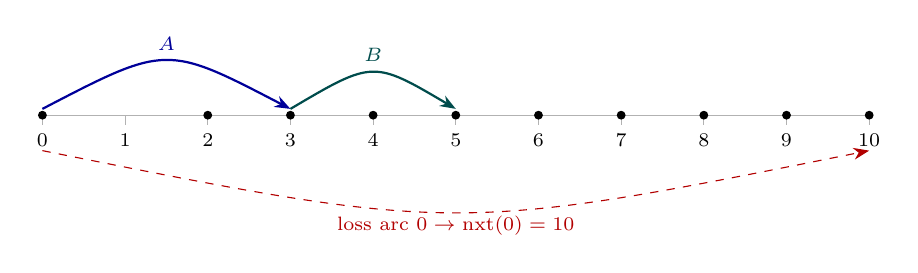
\begin{tikzpicture}[x=1.05cm,y=1cm,>={Stealth[length=2mm]}]
  \foreach \t in {0,...,10} {\draw[gray!60] (\t,0) -- (\t,-0.12) node[below,font=\scriptsize,text=black]{\t};}
  \draw[gray!60] (0,0) -- (10,0);
  \foreach \t in {0,2,3,4,5,6,7,8,9,10} {\fill (\t,0) circle (1.6pt);}
  \draw[->,thick,blue!60!black] (0,0.08) .. controls (1.5,0.9) .. (3,0.08) node[midway,above,font=\scriptsize]{$A$};
  \draw[->,thick,teal!60!black] (3,0.08) .. controls (4,0.7) .. (5,0.08) node[midway,above,font=\scriptsize]{$B$};
  \draw[->,dashed,red!70!black] (0,-0.45) .. controls (5,-1.5) .. (10,-0.45);
  \node[font=\scriptsize,red!70!black] at (5,-1.4) {loss arc $0\to\Nxt(0)=10$};
\end{tikzpicture}
\end{center}

\begin{theorem}[Represent; remove then left-shift; \lean{represent}, \lean{remove\_then\_leftShift}]\label{thm:remove}
Let $P$ be a pattern set with $P\cap[0,H]\subseteq V$.
\begin{enumerate}[label=(\alph*),nosep]
  \item Every capacity-feasible $(J,s)$ admits $s'$ with $r_j\le s'_j\le s_j$,
    $s'_j\in P$, all arcs on nodes, and a compressed flow.
  \item If $(J,s)$ has a compressed flow and $J'\subseteq J$, then
    $(J',s|_{J'})$ need not have one (\cref{ex:removal}), but there is $s'$ on
    $J'$ with $r_j\le s'_j\le s_j$, $s'_j\in P$, and a compressed flow.
\end{enumerate}
\end{theorem}
\begin{proof}
(a) \Cref{thm:ls} gives a left-shifted $s'$ with $r_j\le s'_j\le s_j$;
\cref{thm:pattern} gives $s'_j\in P$, and (P3) gives $s'_j+p_j\in P$; both lie
in $[0,H]$, hence in $V$; \cref{thm:complete} gives the flow. (b) By
\cref{thm:sound} $(J,s)$ is capacity-feasible; removing jobs lowers occupancy
pointwise, so $(J',s)$ is capacity-feasible; apply (a).
\end{proof}

\begin{theorem}\label{thm:N2}
Assume $w\ge0$. $\Rep$ of the N2 model is a $\preceqP$-covering of $\Sched$.
\end{theorem}
\begin{proof}
Soundness: \cref{thm:sound} on each type. Covering: given $\sigma\in\Sched$,
apply \cref{thm:remove}(a) per type; $\mu$ is unchanged and starts only move
earlier.
\end{proof}

%======================================================================
\section{Unbounded types, R1 and R2}\label{sec:R1R2}
%======================================================================

From here on \cref{ass:nonneg} holds; otherwise the code builds the model
with N1/N2 only (if enabled).

\begin{definition}[Unbounded type; \code{unbounded\_types}]
Let $n_m:=|\{j:m\in F_j\}|$. Type $m$ is \emph{unbounded}, $m\in\U$, if
$N_m=\infty$ or $N_m-R_m\ge n_m$. Write $\Mcap:=\M\setminus\U$.
\end{definition}

\begin{lemma}\label{lem:unbounded}
If $m\in\U$, every assignment of jobs to $m$ at any starts in $T$ is
capacity-feasible on $m$.
\end{lemma}
\begin{proof}
$\Run_m(u)+\Busy_m(u)\le R_m+n_m\le N_m$ (or \cref{lem:barN}).
\end{proof}

\begin{lemma}[Relocation]\label{lem:relocate}
Let $\sigma\in\Sched$, $j\in\J$, $k\in\U\cap F_j$, and let $\sigma'$ equal
$\sigma$ except $(\mu'_j,s'_j)=(k,r_j)$. Then $\sigma'\in\Sched$,
$f_1(\sigma')-f_1(\sigma)=w_j\,(r_j+p_{jk}-C_j)$ and
\[
f_2(\sigma')-f_2(\sigma)\le c_{jk}-c_{j\mu_j}+U_k .
\]
If $U_k=0$, the bound is $c_{jk}-c_{j\mu_j}$.
\end{lemma}
\begin{proof}
$r_j\in T_{jk}$ (nonempty, starts at $r_j$). Feasibility on $k$:
\cref{lem:unbounded}. On $\mu_j$ occupancy drops pointwise; other types are
untouched. For $f_2$: $\mu'(\J)\subseteq\mu(\J)\cup\{k\}$, so
$\sum_{\mu'(\J)}U-\sum_{\mu(\J)}U\le U_k\ind{k\notin\mu(\J)}\le U_k$ using
$U\ge0$.
\end{proof}

For $k\in\U\cap F_j$ with $S_{jk}\ne\emptyset$ put
$C_{jk}:=\min S_{jk}+p_{jk}$, the earliest completion on $k$. In all
configurations $\min S_{jk}=r_j$ (the release is in $T_{jk}$ and is a
pattern seed), so $C_{jk}=r_j+p_{jk}$.

\subsection{R1: collapse unbounded types}

\paragraph{Rule.} For $k\in\U$: $S_{jk}:=\{r_j\}$, and $k$ gets no flow
network (no $y$, no rows \eqref{eq:flow}).

\begin{lemma}\label{lem:R1}
Every $\sigma\in\Sched$ has $\sigma'\preceqP\sigma$ in which every job on an
unbounded type starts at its release, and every such $\sigma'$ satisfies all
model constraints involving unbounded types.
\end{lemma}
\begin{proof}
Set $s'_j:=r_j$ whenever $\mu_j\in\U$: feasible by \cref{lem:unbounded},
$f_2$ unchanged, $f_1$ not larger ($w\ge0$). No row of the model mentions an
unbounded type except \eqref{eq:assign} and \eqref{eq:fixed}.
\end{proof}

\subsection{R2: Pareto filter on unbounded options}

\paragraph{Rule.} For job $j$, let $K^0_j:=\{k\in\U\cap F_j:S_{jk}\ne\emptyset\}$.
Scan $K^0_j$ in increasing order of the key $(C_{jk},c_{jk},\ind{U_k>0},k)$
keeping $b:=\min\{c_{jd}: d\text{ kept},\ U_d=0\}$ ($b=\infty$ initially);
keep $k$ iff $c_{jk}<b$. The kept set is $K^2_j$; unbounded options outside
$K^2_j$ are removed.

\begin{lemma}\label{lem:R2}
For every $k\in K^0_j\setminus K^2_j$ there is $d\in K^2_j$ with $U_d=0$,
$C_{jd}\le C_{jk}$, $c_{jd}\le c_{jk}$. Relocating $j$ from $k$ to $(d,r_j)$
gives $\sigma'\preceqP\sigma$. The first element of the scan is always kept,
so $\min_{k\in K^2_j}C_{jk}=\min_{k\in K^0_j}C_{jk}$.
\end{lemma}
\begin{proof}
When $k$ is rejected, $c_{jk}\ge b=c_{jd}$ for a kept $d$ with $U_d=0$ that
was scanned earlier, so $C_{jd}\le C_{jk}$. By \cref{lem:relocate},
$f_1$ changes by $w_j(C_{jd}-C_j)\le w_j(C_{jd}-C_{jk})\le0$ (any start on $k$
completes at $\ge C_{jk}$) and $f_2$ by at most $c_{jd}-c_{jk}\le0$.
\end{proof}

R2 never uses an option with a fixed cost as a dominator, because its
marginal cost depends on whether the type is used by other jobs. Such options
are kept unless an option with $U=0$ dominates them.

%======================================================================
\section{R3: rejection deadlines for weighted sums}\label{sec:R3}
%======================================================================

Hint: \code{objective=(alpha, beta)} with $\alpha,\beta\ge0$; target problems
$\mathrm W(\alpha,\beta,\varepsilon)$.

\paragraph{Scores.} For job $j$ and option $(m,t)$ let
\[
\varphi_j(m,t):=\alpha w_j\,(t+p_{jm}-a_j)+\beta c_{jm},
\]
the job's own contribution to $\alpha f_1+\beta f_2$ without fixed costs. It
is nondecreasing in $t$ because $\alpha w_j\ge0$. For $k\in K^2_j$ let
\[
\rho_{jk}:=\varphi_j(k,r_j)+\beta U_k ,
\]
an upper bound on what placing $j$ on $(k,r_j)$ adds to the scalar objective.

\paragraph{Rule, unbounded part.} Scan $K^2_j$ in increasing order of
$(\rho_{jk},C_{jk},k)$; keep $k$ iff no already-kept $d$ satisfies
$C_{jd}\le C_{jk}$ and $\rho_{jd}\le\varphi_j(k,r_j)$. The kept set is
$K^3_j$.

\paragraph{Rule, capacitated part.} For $m\in\Mcap\cap F_j$ with
$\ell o:=\min S_{jm}$, and $k\in K^3_j$, let
\[
\tau_{jmk}:=\min\{t\in\Z: t\ge \ell o,\ \varphi_j(m,t)\ge\rho_{jk}\}\ (\infty\text{ if empty}),\qquad
\theta_{jmk}:=\max(C_{jk}-p_{jm},\ \tau_{jmk}),
\]
$\Cut_{jm}:=\min_{k\in K^3_j}\theta_{jmk}$, and $S^{3}_{jm}:=\{t\in S_{jm}: t<\Cut_{jm}\}$
(\code{\_first\_start\_reaching}, \code{\_truncate}).

\begin{lemma}[Shape of the deadline]\label{lem:R3shape}
For $t\in S_{jm}$: $t\notin S^3_{jm}$ iff there is $k\in K^3_j$ with
$t+p_{jm}\ge C_{jk}$ and $\varphi_j(m,t)\ge\rho_{jk}$.
\end{lemma}
\begin{proof}
For fixed $k$ and $t\ge \ell o$, $t+p_{jm}\ge C_{jk}\iff t\ge C_{jk}-p_{jm}$,
and, since $\varphi_j(m,\cdot)$ is nondecreasing on integers,
$\varphi_j(m,t)\ge\rho_{jk}\iff t\ge\tau_{jmk}$. So both hold iff
$t\ge\theta_{jmk}$, and some $k$ works iff $t\ge\min_k\theta_{jmk}=\Cut_{jm}$.
\end{proof}

\begin{lemma}[R3 moves]\label{lem:R3move}
Let $\sigma\in\Sched$ and $j$ be placed on an option that R3 removes:
either $(k',r_j)$ with $k'\in K^2_j\setminus K^3_j$, or $(m,t)$ with
$m\in\Mcap$, $t\notin S^3_{jm}$. Then there is $d\in K^3_j$ such that
relocating $j$ to $(d,r_j)$ yields $\sigma'\in\Sched$ with
$\sigma'\preceqW\sigma$.
\end{lemma}
\begin{proof}
In the first case the scan rejected $k'$ because of a kept $d$ with
$C_{jd}\le C_{jk'}$ and $\rho_{jd}\le\varphi_j(k',r_j)$ (rejection compares
only against kept elements, so no chain is needed). In the second case
\cref{lem:R3shape} supplies $d$ with $C_{jd}\le t+p_{jm}$ and
$\rho_{jd}\le\varphi_j(m,t)$. In both cases write $(m_0,t_0)$ for the old
option, so $C_{jd}\le C_j$ and $\rho_{jd}\le\varphi_j(m_0,t_0)$. By
\cref{lem:relocate}, $f_1(\sigma')-f_1(\sigma)=w_j(C_{jd}-C_j)\le0$ and
\[
\alpha\Delta f_1+\beta\Delta f_2\le \alpha w_j(C_{jd}-C_j)+\beta(c_{jd}-c_{jm_0}+U_d)
=\rho_{jd}-\varphi_j(m_0,t_0)\le0 .\qedhere
\]
\end{proof}

\begin{remark}
\begin{enumerate}[nosep]
\item The fixed cost of the \emph{source} is never credited, and the fixed
  cost of the \emph{target} is always charged in full: the bound is
  conservative in both directions, which is what makes the per-job rule
  valid regardless of what the other jobs do.
\item With $\alpha=0$ or $w_j=0$, $\varphi_j(m,\cdot)$ is constant and
  $\tau_{jmk}\in\{\ell o,\infty\}$; the rule still demands $C_{jd}\le C_j$ so
  that f1 caps remain valid.
\item R3 is \emph{not} valid under an upper bound on $f_2$. One job, an
  on-prem option completing at $10$ with $c=0$, a cloud option completing at
  $2$ with $c=1$, $(\alpha,\beta)=(1,1)$, $a_j=0$: the on-prem option has
  score $10\ge\rho=3$ and is removed, so adding $f_2\le\tfrac12$ makes the
  reduced model infeasible while the full one is not.
\end{enumerate}
\end{remark}

%======================================================================
\section{LX: deadlines for the lexicographic objective}\label{sec:LX}
%======================================================================

Hint: \code{objective=LEX\_F1}; target problems $\mathrm L(\varepsilon)$.

\paragraph{Rule.} For every job with $w_j>0$ and $K^2_j\neq\emptyset$ let
$c^\star_j:=\min_{k\in K^2_j}C_{jk}$, the fastest unbounded completion. Keep
only $K^{\mathrm L}_j:=\{k\in K^2_j : C_{jk}=c^\star_j\}$ among unbounded options
and, for $m\in\Mcap$, $S^{\mathrm L}_{jm}:=\{t\in S_{jm}: t+p_{jm}\le c^\star_j\}$.
Jobs with $w_j=0$ are exempt (only R1 and R2 apply to them).

\begin{lemma}[LX moves]\label{lem:LXmove}
Let $\sigma\in\Sched$, $w_j>0$, $K^2_j\ne\emptyset$, and $C_j>c^\star_j$.
Relocating $j$ to $(k^\star,r_j)$ for any $k^\star\in K^{\mathrm L}_j$ yields
$\sigma'\in\Sched$ with $f_1(\sigma')\le f_1(\sigma)-w_j<f_1(\sigma)$; in
particular $\sigma'\preceqL\sigma$.
\end{lemma}
\begin{proof}
\Cref{lem:relocate}: $\Delta f_1=w_j(c^\star_j-C_j)$, and $C_j-c^\star_j\ge1$
because both are integers.
\end{proof}

Every option that LX removes from a job with $w_j>0$ completes after
$c^\star_j$: a capacitated start $t$ with $t+p_{jm}>c^\star_j$, or an
unbounded $k\in K^2_j$ with $C_{jk}>c^\star_j$.

\begin{proposition}[LX keeps all f1-optima]\label{prop:LXall}
Every $f_1$-optimal schedule $\sigma$ over $\{\sigma\in\Sched: f_1\le\varepsilon\}$
satisfies $C_j\le c^\star_j$ for every job with $w_j>0$ and
$K^2_j\ne\emptyset$.
\end{proposition}
\begin{proof}
Otherwise \cref{lem:LXmove} produces a feasible schedule with strictly
smaller $f_1$.
\end{proof}

\begin{proposition}[Tolerance in the second phase]\label{prop:tol}
The code solves $\mathrm L$ as $f_1^\star:=\min f_1$, then $\min f_2$ subject
to $f_1\le f_1^\star+\delta$ with $\delta=10^{-6}$. If
$\delta<w_{\min}:=\min\{w_j:w_j>0\}$, the reduced model gives the same
second-phase value as the full model.
\end{proposition}
\begin{proof}
Let $\sigma\in\Sched$ with $f_1(\sigma)\le f_1^\star+\delta$. If some job
violated its LX deadline, \cref{lem:LXmove} would give
$f_1<f_1^\star+\delta-w_j\le f_1^\star$, impossible. So $\sigma$ violates no
deadline and the remaining steps of the main proof (R1, R2, left shift) give
$\hat\sigma\preceqP\sigma$ in the reduced model.
\end{proof}

The same argument shows the lex rule stays exact with any f1 cap. Like R3 it
is invalid under an f2 cap; the example in the R3 remark applies verbatim.

%======================================================================
\section{The main theorem}\label{sec:main}
%======================================================================

The default configuration is \code{collapse\_unbounded}, \code{pareto\_unbounded},
\code{rejection\_deadlines}, \code{lex\_deadlines} all on, with any choice of
the grid, N1 or N2. The reductions are applied in \code{\_reduce} in the
order R1, R2, then LX (if the hint is \code{LEX\_F1}) or R3 (if the hint is
$(\alpha,\beta)\ge0$), on the start sets $S$ produced by the time-grid choice.

\begin{theorem}[Exactness of the reduced model]\label{thm:main}
Assume \cref{ass:nonneg}. Let $\mathcal M_h$ be the model built with hint
$h$, and let $\preceq_h$ be $\preceqP$ for $h=$\code{None}, $\preceqW$ for
$h=(\alpha,\beta)$, and $\preceqL$ for $h=$\code{LEX\_F1}. Then
$\Rep(\mathcal M_h)\subseteq\Sched$ and $\Rep(\mathcal M_h)$ is a
$\preceq_h$-covering of $\Sched$. Consequently (\cref{lem:covering}),
$\mathcal M_{\texttt{None}}$ is exact for every monotone problem, including
f2 caps and the Pareto front; $\mathcal M_{(\alpha,\beta)}$ is exact for
$\mathrm W(\alpha,\beta,\varepsilon)$; $\mathcal M_{\texttt{LEX\_F1}}$ is
exact for $\mathrm L(\varepsilon)$.
\end{theorem}

\begin{proof}
\emph{Soundness.} Rows \eqref{eq:assign} make $x$ a schedule whose options lie
in $S\subseteq T$. Each type with a flow network is capacity-feasible by
\cref{thm:grid} (grid, N1) or \cref{thm:sound} (N2). Types without a flow
network are unbounded and capacity-feasible by \cref{lem:unbounded}. With
\cref{lem:fixed}, $\Rep(\mathcal M_h)\subseteq\Sched$ and the model's
objectives are the true ones.

\emph{Covering.} Let $\sigma\in\Sched$. We build $\hat\sigma\in\Rep(\mathcal M_h)$
with $\hat\sigma\preceq_h\sigma$ in four stages. Each stage changes one job at a
time and produces a schedule in $\Sched$ that is $\preceq_h$ the previous
one; by transitivity the final schedule is $\preceq_h\sigma$.
\begin{enumerate}[label=\textbf{Stage \arabic*.},leftmargin=*]
\item (R1) Move every job on an unbounded type to its release
  (\cref{lem:R1}); $\preceqP$, hence $\preceq_h$.
\item (R2) Relocate every job sitting on an unbounded option outside
  $K^2_j$ to its dominator $d\in K^2_j$ (\cref{lem:R2}); $\preceqP$. Now every
  job on an unbounded type sits at $(k,r_j)$ with $k\in K^2_j$.
\item (Hint-specific.) For $h=(\alpha,\beta)$: relocate every job on an
  option removed by R3 to the $d\in K^3_j$ of \cref{lem:R3move};
  $\preceqW$. For $h=$\code{LEX\_F1}: relocate every job with $w_j>0$,
  $K^2_j\ne\emptyset$ and $C_j>c^\star_j$ to some $k^\star\in K^{\mathrm L}_j$
  (\cref{lem:LXmove}); $\preceqL$. After this stage, every job on an
  unbounded type sits on an option the model keeps, and every job on a
  capacitated type $m$ has its \emph{original} start $s_j$, which satisfies
  $s_j\in T_{jm}$ and the deadline ($s_j<\Cut_{jm}$, resp.
  $s_j+p_{jm}\le c^\star_j$), because jobs violating it were relocated.
  Relocations only \emph{remove} jobs from capacitated types.
\item (Representation on capacitated types.) For the grid model, the
  schedule is already represented (\cref{thm:grid}). For N1 or N2, apply
  \cref{thm:ls,thm:pattern} (resp. \cref{thm:remove}(a)) on each
  capacitated type: starts move to $s'_j\in P_m$ with $r_j\le s'_j\le s_j$
  and, for N2, a compressed flow exists. Every deadline set is
  \emph{down-closed} on $[r_j,\infty)$, so $s'_j$ still satisfies it, and
  $s'_j+p_{jm}\le s_j+p_{jm}\le H$. $\mu$ is unchanged, $f_2$ is unchanged and
  $f_1$ does not increase: $\preceqP$.
\end{enumerate}
The final schedule uses only options in the reduced sets, every flow type has
a flow (and $y$ or $\ell$ exist), and $z$ is set by \cref{lem:fixed}; so it
lies in $\Rep(\mathcal M_h)$.
\end{proof}

\begin{remark}[Other flag combinations]
Each flag can be turned off independently. Without R1, unbounded types keep
all their starts and their flow network; stage 1 is skipped and stage 4 runs
on unbounded types too (\cref{thm:ls} applies to any finite $\bar N$). The
comparisons of R2, R3 and LX use $C_{jk}=r_j+p_{jk}$, a lower bound on the
completion of every start on $k$, and the relocation target $(d,r_j)$ is
still in the model, so the same proof goes through. Without R2, use
$K^2_j:=K^0_j$.
\end{remark}

\begin{remark}[Why stage 4 is needed]
\Cref{ex:removal} shows that stage 3 may leave a capacitated type with a
schedule that has no compressed flow. Stage 4 repairs this. The repair cannot
violate a deadline because it only moves starts earlier; this is the reason
every deadline in R3 and LX is an upper bound on the start.
\end{remark}

\subsection{Validity per hint and caller contract}

\begin{center}
\begin{tabular}{@{}lll@{}}
\toprule
Problem & Hint to pass & Active rules\\
\midrule
$\min\alpha f_1+\beta f_2$, optional $f_1\le\varepsilon$ & $(\alpha,\beta)$, $\alpha,\beta\ge0$ & N1/N2, R1, R2, R3\\
lex $(f_1,f_2)$, optional $f_1\le\varepsilon$ & \code{LEX\_F1} & N1/N2, R1, R2, LX\\
any problem with an $f_2$ cap, Pareto front, box search & \code{None} & N1/N2, R1, R2\\
\bottomrule
\end{tabular}
\end{center}

A model built with a hint is valid only for that hint's problem family
(the returned key \code{objective\_reduced} records that one ran). The current callers
respect this: \code{pareto.py} passes \code{LEX\_F1} only when the bound is
absent or on $f_1$; \code{solve\_epsilon\_cost} and the Pareto steps pass
\code{None}; \code{rm\_benchmark} passes $(1,1)$ for a weighted sum. No caller
maximises.

%======================================================================
\section{State of the proofs}\label{sec:status}
%======================================================================

\subsection{Machine-checked (Lean 4 + Mathlib)}

\code{proofs/Proofs/CompressedFlow.lean} (650 lines) builds with
\code{lake build}; \code{\#print axioms Fedhpc.Graph.remove\_then\_leftShift}
reports only \code{propext}, \code{Classical.choice}, \code{Quot.sound}; there
is no \code{sorry}. The model is one finite-capacity type
(\lean{TypeInst}: $H>0$, $N$, jobs with \lean{rel}~$=r_j$ and $p\ge1$, running
ends $\le H$, $R\le N$) and one graph (\lean{Graph}: $E\subseteq V$,
$0,H\in E$, releases and running ends in $E$, $V\subseteq[0,H]$, \lean{nxt}
the next event).

\begin{center}
\begin{tabular}{@{}l>{\raggedright\arraybackslash}p{0.68\textwidth}@{}}
\toprule
This document & Lean\\
\midrule
\Cref{lem:recurrences} & \lean{run\_succ}, \lean{busy\_succ}, \lean{run\_zero}, \lean{busy\_zero}, \lean{ends\_zero}, \lean{run\_last}, \lean{busy\_last}, \lean{starts\_last}\\
\Cref{thm:ls} & \lean{exists\_leftShift}\\
\Cref{thm:pattern} & \lean{leftShifted\_mem\_pattern}\\
\Cref{lem:arcs} & \lean{arcIdle\_zero}, \lean{arc\_succ}, \lean{inLoss\_of\_not\_mem\_E}, \lean{inLoss\_of\_mem\_E}\\
\Cref{thm:sound} & \lean{invariant}, \lean{sound} ($\ell\in\N$), \lean{invariantR}, \lean{soundR} ($\ell\in\R_{\ge0}$)\\
\Cref{lem:idlemono} & \lean{idle\_mono}\\
\Cref{thm:complete} & \lean{lossOf}, \lean{arcIdle\_lossOf}, \lean{complete}\\
\Cref{thm:remove} & \lean{represent}, \lean{remove\_then\_leftShift}\\
\bottomrule
\end{tabular}
\end{center}

\subsection{Proved on paper only (this document)}

\begin{enumerate}[label=(\roman*)]
\item \Cref{lem:covering} (coverings preserve optima and the Pareto front).
\item \Cref{thm:grid} (grid flow $\Leftrightarrow$ capacity). Soundness is the
  Lean \lean{sound} with $E=V=[0,H]$; Lean's \lean{complete} assumes a
  left-shifted schedule, which the grid does not need, so completeness for
  arbitrary schedules is not machine-checked.
\item \Cref{lem:fixed} (fixed-cost linking), \cref{lem:unbounded,lem:relocate}.
\item The reduction lemmas \cref{lem:R1,lem:R2,lem:R3shape,lem:R3move,lem:LXmove},
  \cref{prop:LXall,prop:tol}, and the composition \cref{thm:main}, including
  the multi-type decomposition and the assignment rows.
\item \Cref{lem:computedP} (the code's grouped closure is a pattern set) and
  the upper bound $\ell\le\bar N$ in \cref{thm:complete}, which the Lean
  \lean{Conserve} omits (it holds since $\ell_q\le\Idle(q)\le\bar N$).
\end{enumerate}

\subsection{Tested, not proved}

\begin{itemize}
\item \emph{Fidelity of the code to the rules stated here}: scan orders and
  tie-breaking in \code{\_reduce}, \code{\_first\_start\_reaching},
  \code{\_truncate}, and the C++ graph builder against the Python fallback
  (\code{test\_cpp\_graph\_builder\_matches\_python\_fallback}).
\item \emph{Brute-force oracle} (\code{tests/test\_spacetime\_oracle.py}):
  12 random instances with 4 jobs and $H=11$, two capacitated types, one type
  at exactly the unbounded threshold, 2--3 cloud types with ties, a fixed cost
  on one cloud type, running jobs and weights in $\{0,1,2,3\}$. All
  schedules are enumerated without any flow model. Checked: lex optima and six
  weight pairs for the grid, N1 and N2; f1-capped weighted sums; lex under an
  f1 cap; the full Pareto front; f2 caps. It caught all three mutations seeded
  into the reductions. Together with \code{test\_spacetime\_reductions.py} and
  \code{test\_spacetime\_options.py}: 168 tests pass (re-run 16 Oct 2026).
\end{itemize}

\subsection{Open points}

\begin{enumerate}[label=G\arabic*.]
\item \textbf{Floating point in R3.} $\varphi$, $\rho$ and $\tau$ are computed
  in double precision with no margin. A start whose exact score is below
  $\rho_{jk}$ by a rounding error may be removed. The loss is bounded by that
  rounding error (about $10^{-15}$ relative), so R3 is exact up to rounding.
  R1, R2 and LX compare integers or the same floats Gurobi sees, and are exact.
\item \textbf{N1/N2 require $w\ge0$ but are not gated by it.}
  \code{normal\_patterns}/\code{compressed\_flow} are applied even when
  \code{nonnegative\_data} is false. With a negative weight, a left shift can
  increase $f_1$ and the restriction can cut the optimum.
\item \textbf{LX tolerance.} Exact when $\delta=10^{-6}<w_{\min}$
  (\cref{prop:tol}); an implicit assumption.
\item \textbf{\code{cover\_ge} docstring} overclaims (\cref{prop:coverge}).
\item \textbf{Coverage gaps of the oracle}: no fixed cost on a capacitated
  type, horizons $\le11$, no adversarial float ties for R3.
\item \textbf{Formalisation}: items (i)--(v) above. The hard combinatorial
  step (stage 4) is already in Lean; the remaining statements are
  per-job inequalities plus bookkeeping across types, and would be a
  moderate extension of \code{CompressedFlow.lean}.
\end{enumerate}

\end{document}
